\section{Tutorial: A Petri-Net for Hagen}

\subsection{Overview}

The expected outcome of this tutorial:
\begin{figure}[H]
    \includegraphics[width=\textwidth]{petrinet_for_hagen/figures/overview.PNG}
    \caption{Expected outcome but in Tikz.}
\end{figure}

\subsection{Execution}

Additional packages needed: \texttt{\textbackslash usetikzlibrary\{arrows,snakes,backgrounds\}}

\vspace{1cm}

\begin{tikzpicture}
    \path ( 0,2) node[shape=circle,draw] {}
          ( 0,1) node[shape=circle,draw] {}
          ( 0,0) node[shape=circle,draw] {}
          ( 1,1) node[shape=rectangle,draw] {}
          (-1,1) node[shape=rectangle,draw] {};
\end{tikzpicture}

\vspace{1cm}

\begin{tikzpicture}
    \path node at ( 0,2) [shape=circle,draw] {}
          node at ( 0,1) [shape=circle,draw] {}
          node at ( 0,0) [shape=circle,draw] {}
          node at ( 1,1) [shape=rectangle,draw] {}
          node at (-1,1) [shape=rectangle,draw] {};
\end{tikzpicture}

\vspace{1cm}

The \texttt{\textbackslash node} command is an abbreviation of \texttt{\textbackslash path node}.

\vspace{1cm}

\begin{tikzpicture}
    \node at ( 0,2) [circle,draw] {};
    \node at ( 0,1) [circle,draw] {};
    \node at ( 0,0) [circle,draw] {};
    \node at ( 1,1) [rectangle,draw] {};
    \node at (-1,1) [rectangle,draw] {};
\end{tikzpicture}

\vspace{1cm}

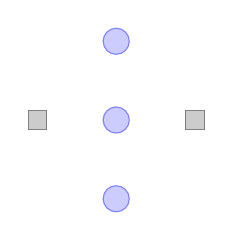
\begin{tikzpicture}
    \node at ( 0,2) [circle,draw=blue!50,fill=blue!20] {};
    \node at ( 0,1) [circle,draw=blue!50,fill=blue!20] {};
    \node at ( 0,0) [circle,draw=blue!50,fill=blue!20] {};
    \node at ( 1,1) [rectangle,draw=black!50,fill=black!20] {};
    \node at (-1,1) [rectangle,draw=black!50,fill=black!20] {};
\end{tikzpicture}

\vspace{1cm}

\tikzstyle{place} = [circle,draw=blue!50,fill=blue!20,thick]
\tikzstyle{transition} = [rectangle,draw=black!50,fill=black!20,thick]

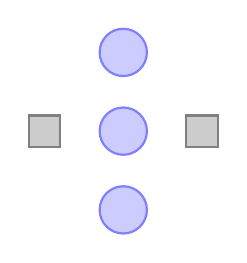
\begin{tikzpicture}
    \node at ( 0,2) [place] {};
    \node at ( 0,1) [place] {};
    \node at ( 0,0) [place] {};
    \node at ( 1,1) [transition] {};
    \node at (-1,1) [transition] {};
\end{tikzpicture}

\vspace{1cm}

\tikzstyle{place} = [circle,draw=blue!50,fill=blue!20,thick]
\tikzstyle{transition} = [rectangle,draw=black!50,fill=black!20,thick]

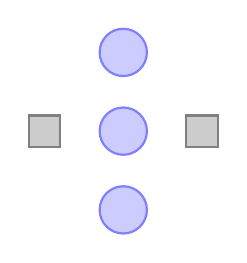
\begin{tikzpicture}[inner sep=2mm]
    \node at ( 0,2) [place] {};
    \node at ( 0,1) [place] {};
    \node at ( 0,0) [place] {};
    \node at ( 1,1) [transition] {};
    \node at (-1,1) [transition] {};
\end{tikzpicture}

\vspace{1cm}

\tikzstyle{place} = [circle,draw=blue!50,fill=blue!20,thick]
\tikzstyle{transition} = [rectangle,draw=black!50,fill=black!20,thick]

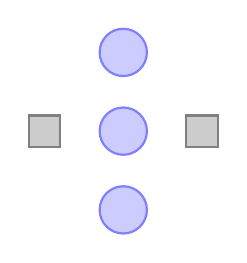
\begin{tikzpicture}[inner sep=2mm]
    \node at ( 0,2) [place] {};
    \node at ( 0,1) [place] {};
    \node at ( 0,0) [place] {};
    \node at ( 1,1) [transition] {};
    \node at (-1,1) [transition] {};
\end{tikzpicture}

\vspace{1cm}

\tikzstyle{place} = [circle,draw=blue!50,fill=blue!20,thick,inner sep=0mm,minimum size=6mm]
\tikzstyle{transition} = [rectangle,draw=black!50,fill=black!20,thick,inner sep=0mm,minimum size=4mm]

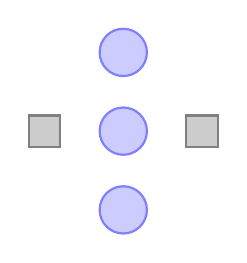
\begin{tikzpicture}[ ]
    \node at ( 0,2) [place] {};
    \node at ( 0,1) [place] {};
    \node at ( 0,0) [place] {};
    \node at ( 1,1) [transition] {};
    \node at (-1,1) [transition] {};
\end{tikzpicture}

\vspace{1cm}

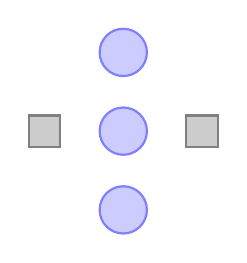
\begin{tikzpicture}[ ]
    \node (waiting 1)   at ( 0,2) [place] {};
    \node (critical 1)  at ( 0,1) [place] {};
    \node (semaphore)   at ( 0,0) [place] {};
    \node (leave critical)  at ( 1,1) [transition] {};
    \node (enter critical)  at (-1,1) [transition] {};
\end{tikzpicture}

\vspace{1cm}

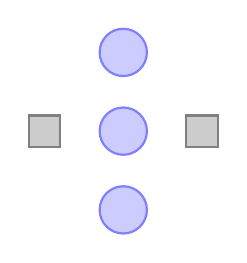
\begin{tikzpicture}[ ]
    \node[place] (waiting 1)            at ( 0,2) {};
    \node[place] (critical 1)           at ( 0,1) {};
    \node[place] (semaphore)            at ( 0,0) {};
    \node[transition] (leave critical)  at ( 1,1) {};
    \node[transition] (enter critical)  at (-1,1) {};
\end{tikzpicture}

\vspace{1cm}

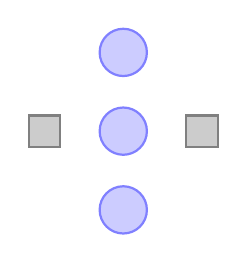
\begin{tikzpicture}[ ]
    \node[place] (waiting)                                  {};
    \node[place] (critical)             [below of=waiting]  {};
    \node[place] (semaphore)            [below of=critical] {};
    \node[transition] (leave critical)  [right of=critical] {};
    \node[transition] (enter critical)  [left of=critical]  {};
\end{tikzpicture}

\vspace{1cm}

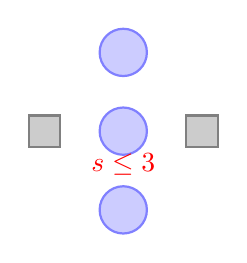
\begin{tikzpicture}[ ]
    \node[place] (waiting)                                  {};
    \node[place] (critical)             [below of=waiting]  {};
    \node[place] (semaphore)            [below of=critical] {};
    \node[transition] (leave critical)  [right of=critical] {};
    \node[transition] (enter critical)  [left of=critical]  {};

    \node[red,above] at (semaphore.north) {$s\le 3$};
\end{tikzpicture}

\vspace{1cm}
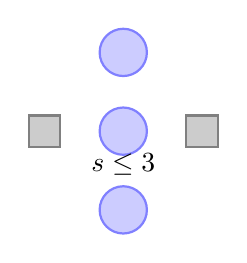
\begin{tikzpicture}[ ]
    \node[place] (waiting)                                  {};
    \node[place] (critical)             [below of=waiting]  {};
    \node[place] (semaphore)            [below of=critical,
                                         label=above:$s\le 3$] {};
    \node[transition] (leave critical)  [right of=critical] {};
    \node[transition] (enter critical)  [left of=critical]  {};
\end{tikzpicture}

\vspace{1cm}

\tikz
    \node[circle,draw,
          label=60:$60^\circ$,
          label=270:$-90^\circ$] {my circle};

\vspace{1cm}

\vspace{1cm}

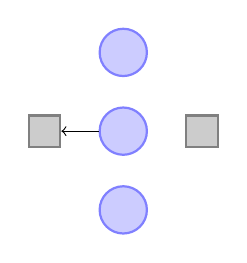
\begin{tikzpicture}[ ]
    \node[place] (waiting)                                  {};
    \node[place] (critical)             [below of=waiting]  {};
    \node[place] (semaphore)            [below of=critical] {};
    \node[transition] (leave critical)  [right of=critical] {};
    \node[transition] (enter critical)  [left of=critical]  {};

    \draw[->] (critical.west) -- (enter critical.east);
\end{tikzpicture}

\vspace{1cm}

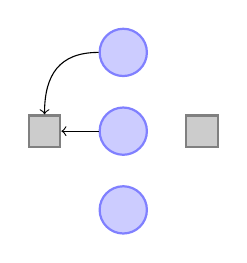
\begin{tikzpicture}[ ]
    \node[place] (waiting)                                  {};
    \node[place] (critical)             [below of=waiting]  {};
    \node[place] (semaphore)            [below of=critical] {};
    \node[transition] (leave critical)  [right of=critical] {};
    \node[transition] (enter critical)  [left of=critical]  {};

    \draw[->] (critical.west) -- (enter critical.east);
    \draw[->] (waiting.west) .. controls +(left:5mm) and +(up:5mm) .. (enter critical.north);
\end{tikzpicture}

\vspace{1cm}

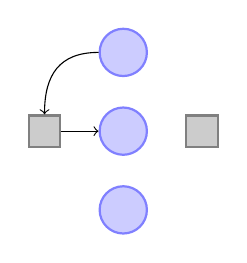
\begin{tikzpicture}[ ]
    \node[place] (waiting)                                  {};
    \node[place] (critical)             [below of=waiting]  {};
    \node[place] (semaphore)            [below of=critical] {};
    \node[transition] (leave critical)  [right of=critical] {};
    \node[transition] (enter critical)  [left of=critical]  {};

    \draw[->] (enter critical) -- (critical);
    \draw[->] (waiting.west) .. controls +(left:5mm) and +(up:5mm) .. (enter critical.north);
\end{tikzpicture}

\vspace{1cm}

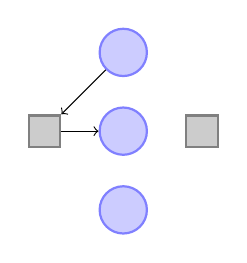
\begin{tikzpicture}[ ]
    \node[place] (waiting)                                  {};
    \node[place] (critical)             [below of=waiting]  {};
    \node[place] (semaphore)            [below of=critical] {};
    \node[transition] (leave critical)  [right of=critical] {};
    \node[transition] (enter critical)  [left of=critical]  {};

    \draw[->] (enter critical)  to (critical);
    \draw[->] (waiting)         to (enter critical);
\end{tikzpicture}

\vspace{1cm}

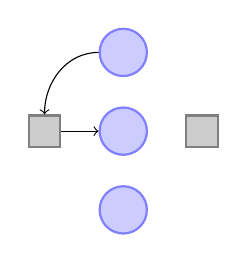
\begin{tikzpicture}[ ]
    \node[place] (waiting)                                  {};
    \node[place] (critical)             [below of=waiting]  {};
    \node[place] (semaphore)            [below of=critical] {};
    \node[transition] (leave critical)  [right of=critical] {};
    \node[transition] (enter critical)  [left of=critical]  {};

    \draw[->] (enter critical)  to (critical);
    \draw[->] (waiting)         to [out=180,in=90] (enter critical);
\end{tikzpicture}

\vspace{1cm}

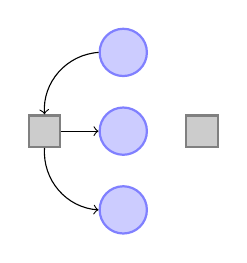
\begin{tikzpicture}[ ]
    \node[place] (waiting)                                  {};
    \node[place] (critical)             [below of=waiting]  {};
    \node[place] (semaphore)            [below of=critical] {};
    \node[transition] (leave critical)  [right of=critical] {};
    \node[transition] (enter critical)  [left of=critical]  {};

    \draw[->] (enter critical)  to (critical);
    \draw[->] (waiting)         to [bend right=45] (enter critical);
    \draw[->] (enter critical)  to [bend right=45] (semaphore);
\end{tikzpicture}

\vspace{1cm}

\tikzstyle{pre} = [<-,shorten <= 1pt,>=stealth',semithick]
\tikzstyle{post} = [->,shorten >= 1pt,>=stealth',semithick]

\begin{tikzpicture}[bend angle=45]
    \node[place] (waiting)                                  {};
    \node[place] (critical)             [below of=waiting]  {};
    \node[place] (semaphore)            [below of=critical] {};
    
    \node[transition] (leave critical)  [right of=critical] {}
        edge[pre] (critical)
        edge[post,bend right] (waiting)
        edge[pre,bend left] (semaphore);
    \node[transition] (enter critical)  [left of=critical]  {}
        edge[post]              (critical)
        edge[pre,bend left]     (waiting)
        edge[post,bend right]    (semaphore);
\end{tikzpicture}

\subsubsection{Adding labels next to lines}

\vspace{1cm}

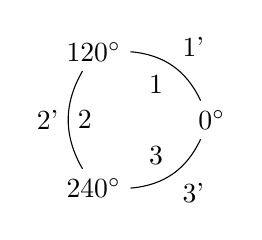
\begin{tikzpicture}[auto,bend right]
    \node (a) at (0:1) {$0^\circ$};
    \node (b) at (120:1) {$120^\circ$};
    \node (c) at (240:1) {$240^\circ$};

    \draw (a) to node {1} node[swap] {1'} (b)
          (b) to node {2} node[swap] {2'} (c)
          (c) to node {3} node[swap] {3'} (a);
\end{tikzpicture}

\vspace{1cm}

\begin{tikzpicture}[bend angle=45]
    \node[place] (waiting)                                  {};
    \node[place] (critical)             [below of=waiting]  {};
    \node[place] (semaphore)            [below of=critical] {};
    
    \node[transition] (leave critical)  [right of=critical] {}
        edge[pre] (critical)
        edge[post,bend right] node[auto,swap] {2} (waiting)
        edge[pre,bend left] (semaphore);
    \node[transition] (enter critical)  [left of=critical]  {}
        edge[post]              (critical)
        edge[pre,bend left]     (waiting)
        edge[post,bend right]    (semaphore);
\end{tikzpicture}

\subsubsection{Adding the snaked line and multi-line text}

\vspace{1cm}

\begin{tikzpicture}
    \draw[->,snake=snake] (0,0) -- (2,0);
\end{tikzpicture}

\vspace{1cm}

\begin{tikzpicture}
    \draw[->,snake=snake,
          segment amplitude=.4mm,
          segment length=2mm,
          line after snake=1mm] (0,0) -- (2,0);
\end{tikzpicture}

\vspace{1cm}

\begin{tikzpicture}
    \draw[->,snake=snake,
          segment amplitude=.4mm,
          segment length=2mm,
          line after snake=1mm] (0,0) -- (3,0)
        node[above,text width=3cm,text centered,midway]
        {
            replacement of the \textcolor{red}{capacity} by \textcolor{red}{two places}
        };
\end{tikzpicture}

\subsubsection{Using layers: the background rectangles}

\vspace{1cm}

\begin{tikzpicture}[bend angle=45]
    \node[place] (waiting)                                  {};
    \node[place] (critical)             [below of=waiting]  {};
    \node[place] (semaphore)            [below of=critical] {};
    
    \node[transition] (leave critical)  [right of=critical] {}
        edge[pre] (critical)
        edge[post,bend right] node[auto,swap] {2} (waiting)
        edge[pre,bend left] (semaphore);
    \node[transition] (enter critical)  [left of=critical]  {}
        edge[post]              (critical)
        edge[pre,bend left]     (waiting)
        edge[post,bend right]    (semaphore);

    % Background
    \begin{pgfonlayer}{background}
        \filldraw[fill=black!30,draw=red]
                      (semaphore.south -| enter critical.west)
            rectangle (waiting.north -| leave critical.east);
    \end{pgfonlayer}
        
\end{tikzpicture}

\subsubsection{The complete code}

